%% bare_jrnl.tex
%% V1.4b
%% 2015/08/26
%% by Michael Shell
%% see http://www.michaelshell.org/
%% for current contact information.
%%
%% This is a skeleton file demonstrating the use of IEEEtran.cls
%% (requires IEEEtran.cls version 1.8b or later) with an IEEE
%% journal paper.
%%
%% Support sites:
%% http://www.michaelshell.org/tex/ieeetran/
%% http://www.ctan.org/pkg/ieeetran
%% and
%% http://www.ieee.org/

%%*************************************************************************
%% Legal Notice:
%% This code is offered as-is without any warranty either expressed or
%% implied; without even the implied warranty of MERCHANTABILITY or
%% FITNESS FOR A PARTICULAR PURPOSE! 
%% User assumes all risk.
%% In no event shall the IEEE or any contributor to this code be liable for
%% any damages or losses, including, but not limited to, incidental,
%% consequential, or any other damages, resulting from the use or misuse
%% of any information contained here.
%%
%% All comments are the opinions of their respective authors and are not
%% necessarily endorsed by the IEEE.
%%
%% This work is distributed under the LaTeX Project Public License (LPPL)
%% ( http://www.latex-project.org/ ) version 1.3, and may be freely used,
%% distributed and modified. A copy of the LPPL, version 1.3, is included
%% in the base LaTeX documentation of all distributions of LaTeX released
%% 2003/12/01 or later.
%% Retain all contribution notices and credits.
%% ** Modified files should be clearly indicated as such, including  **
%% ** renaming them and changing author support contact information. **
%%*************************************************************************


% *** Authors should verify (and, if needed, correct) their LaTeX system  ***
% *** with the testflow diagnostic prior to trusting their LaTeX platform ***
% *** with production work. The IEEE's font choices and paper sizes can   ***
% *** trigger bugs that do not appear when using other class files.       ***                          ***
% The testflow support page is at:
% http://www.michaelshell.org/tex/testflow/



\documentclass[journal]{IEEEtran}
\usepackage[brazilian]{babel}
\usepackage[utf8]{inputenc}
\usepackage[T1]{fontenc}
\usepackage{algorithm}
\usepackage{algpseudocode}
\usepackage{listings}
\usepackage{float}
\usepackage{color}

\floatname{algorithm}{Código}
\algrenewcommand\algorithmicfunction{\textbf{function}}
\algrenewtext{EndFunction}{\algorithmicend}
\algrenewtext{EndIf}{\algorithmicend}


\definecolor{mygreen}{rgb}{0,0.6,0}
\definecolor{mygray}{rgb}{0.5,0.5,0.5}
\definecolor{mymauve}{rgb}{0.58,0,0.82}

\lstset{ %
  backgroundcolor=\color{white},   % choose the background color; you must add \usepackage{color} or \usepackage{xcolor}; should come as last argument
  basicstyle=\footnotesize,        % the size of the fonts that are used for the code
  breakatwhitespace=false,         % sets if automatic breaks should only happen at whitespace
  breaklines=true,                 % sets automatic line breaking
  % captionpos=a,                    % sets the caption-position to bottom
  % commentstyle=\color{mygreen},    % comment style
  deletekeywords={...},            % if you want to delete keywords from the given language
  escapeinside={\%*}{*)},          % if you want to add LaTeX within your code
  extendedchars=true,              % lets you use non-ASCII characters; for 8-bits encodings only, does not work with UTF-8
  % frame=single,	                   % adds a frame around the code
  keepspaces=true,                 % keeps spaces in text, useful for keeping indentation of code (possibly needs columns=flexible)
  % keywordstyle=\color{blue},       % keyword style
  language=Octave,                 % the language of the code
  morekeywords={*,...},            % if you want to add more keywords to the set
  numbers=left,                    % where to put the line-numbers; possible values are (none, left, right)
  numbersep=-5pt,                   % how far the line-numbers are from the code
  numberstyle=\tiny\color{mygray}, % the style that is used for the line-numbers
  rulecolor=\color{black},         % if not set, the frame-color may be changed on line-breaks within not-black text (e.g. comments (green here))
  showspaces=false,                % show spaces everywhere adding particular underscores; it overrides 'showstringspaces'
  showstringspaces=false,          % underline spaces within strings only
  showtabs=false,                  % show tabs within strings adding particular underscores
  % stepnumber=2,                    % the step between two line-numbers. If it's 1, each line will be numbered
  % stringstyle=\color{mymauve},     % string literal style
  % tabsize=2,	                   % sets default tabsize to 2 spaces
  title=\lstname                   % show the filename of files included with \lstinputlisting; also try caption instead of title
}

%
% If IEEEtran.cls has not been installed into the LaTeX system files,
% manually specify the path to it like:
% \documentclass[journal]{../sty/IEEEtran}





% Some very useful LaTeX packages include:
% (uncomment the ones you want to load)


% *** MISC UTILITY PACKAGES ***
%
%\usepackage{ifpdf}
% Heiko Oberdiek's ifpdf.sty is very useful if you need conditional
% compilation based on whether the output is pdf or dvi.
% usage:
% \ifpdf
%   % pdf code
% \else
%   % dvi code
% \fi
% The latest version of ifpdf.sty can be obtained from:
% http://www.ctan.org/pkg/ifpdf
% Also, note that IEEEtran.cls V1.7 and later provides a builtin
% \ifCLASSINFOpdf conditional that works the same way.
% When switching from latex to pdflatex and vice-versa, the compiler may
% have to be run twice to clear warning/error messages.






% *** CITATION PACKAGES ***
%
%\usepackage{cite}
% cite.sty was written by Donald Arseneau
% V1.6 and later of IEEEtran pre-defines the format of the cite.sty package
% \cite{} output to follow that of the IEEE. Loading the cite package will
% result in citation numbers being automatically sorted and properly
% "compressed/ranged". e.g., [1], [9], [2], [7], [5], [6] without using
% cite.sty will become [1], [2], [5]--[7], [9] using cite.sty. cite.sty's
% \cite will automatically add leading space, if needed. Use cite.sty's
% noadjust option (cite.sty V3.8 and later) if you want to turn this off
% such as if a citation ever needs to be enclosed in parenthesis.
% cite.sty is already installed on most LaTeX systems. Be sure and use
% version 5.0 (2009-03-20) and later if using hyperref.sty.
% The latest version can be obtained at:
% http://www.ctan.org/pkg/cite
% The documentation is contained in the cite.sty file itself.






% *** GRAPHICS RELATED PACKAGES ***
%
\ifCLASSINFOpdf
  \usepackage[pdftex]{graphicx}
  % declare the path(s) where your graphic files are
  \graphicspath{{./img/}}
  % and their extensions so you won't have to specify these with
  % every instance of \includegraphics
  \DeclareGraphicsExtensions{.pdf,.jpg,.jpeg,.png}
\else
  % or other class option (dvipsone, dvipdf, if not using dvips). graphicx
  % will default to the driver specified in the system graphics.cfg if no
  % driver is specified.
  % \usepackage[dvips]{graphicx}
  % declare the path(s) where your graphic files are
  % \graphicspath{{../eps/}}
  % and their extensions so you won't have to specify these with
  % every instance of \includegraphics
  % \DeclareGraphicsExtensions{.eps}
\fi
% graphicx was written by David Carlisle and Sebastian Rahtz. It is
% required if you want graphics, photos, etc. graphicx.sty is already
% installed on most LaTeX systems. The latest version and documentation
% can be obtained at: 
% http://www.ctan.org/pkg/graphicx
% Another good source of documentation is "Using Imported Graphics in
% LaTeX2e" by Keith Reckdahl which can be found at:
% http://www.ctan.org/pkg/epslatex
%
% latex, and pdflatex in dvi mode, support graphics in encapsulated
% postscript (.eps) format. pdflatex in pdf mode supports graphics
% in .pdf, .jpeg, .png and .mps (metapost) formats. Users should ensure
% that all non-photo figures use a vector format (.eps, .pdf, .mps) and
% not a bitmapped formats (.jpeg, .png). The IEEE frowns on bitmapped formats
% which can result in "jaggedy"/blurry rendering of lines and letters as
% well as large increases in file sizes.
%
% You can find documentation about the pdfTeX application at:
% http://www.tug.org/applications/pdftex





% *** MATH PACKAGES ***
%
%\usepackage{amsmath}
% A popular package from the American Mathematical Society that provides
% many useful and powerful commands for dealing with mathematics.
%
% Note that the amsmath package sets \interdisplaylinepenalty to 10000
% thus preventing page breaks from occurring within multiline equations. Use:
%\interdisplaylinepenalty=2500
% after loading amsmath to restore such page breaks as IEEEtran.cls normally
% does. amsmath.sty is already installed on most LaTeX systems. The latest
% version and documentation can be obtained at:
% http://www.ctan.org/pkg/amsmath





% *** SPECIALIZED LIST PACKAGES ***
%
%\usepackage{algorithmic}
% algorithmic.sty was written by Peter Williams and Rogerio Brito.
% This package provides an algorithmic environment fo describing algorithms.
% You can use the algorithmic environment in-text or within a figure
% environment to provide for a floating algorithm. Do NOT use the algorithm
% floating environment provided by algorithm.sty (by the same authors) or
% algorithm2e.sty (by Christophe Fiorio) as the IEEE does not use dedicated
% algorithm float types and packages that provide these will not provide
% correct IEEE style captions. The latest version and documentation of
% algorithmic.sty can be obtained at:
% http://www.ctan.org/pkg/algorithms
% Also of interest may be the (relatively newer and more customizable)
% algorithmicx.sty package by Szasz Janos:
% http://www.ctan.org/pkg/algorithmicx




% *** ALIGNMENT PACKAGES ***
%
%\usepackage{array}
% Frank Mittelbach's and David Carlisle's array.sty patches and improves
% the standard LaTeX2e array and tabular environments to provide better
% appearance and additional user controls. As the default LaTeX2e table
% generation code is lacking to the point of almost being broken with
% respect to the quality of the end results, all users are strongly
% advised to use an enhanced (at the very least that provided by array.sty)
% set of table tools. array.sty is already installed on most systems. The
% latest version and documentation can be obtained at:
% http://www.ctan.org/pkg/array


% IEEEtran contains the IEEEeqnarray family of commands that can be used to
% generate multiline equations as well as matrices, tables, etc., of high
% quality.




% *** SUBFIGURE PACKAGES ***
%\ifCLASSOPTIONcompsoc
%  \usepackage[caption=false,font=normalsize,labelfont=sf,textfont=sf]{subfig}
%\else
%  \usepackage[caption=false,font=footnotesize]{subfig}
%\fi
% subfig.sty, written by Steven Douglas Cochran, is the modern replacement
% for subfigure.sty, the latter of which is no longer maintained and is
% incompatible with some LaTeX packages including fixltx2e. However,
% subfig.sty requires and automatically loads Axel Sommerfeldt's caption.sty
% which will override IEEEtran.cls' handling of captions and this will result
% in non-IEEE style figure/table captions. To prevent this problem, be sure
% and invoke subfig.sty's "caption=false" package option (available since
% subfig.sty version 1.3, 2005/06/28) as this is will preserve IEEEtran.cls
% handling of captions.
% Note that the Computer Society format requires a larger sans serif font
% than the serif footnote size font used in traditional IEEE formatting
% and thus the need to invoke different subfig.sty package options depending
% on whether compsoc mode has been enabled.
%
% The latest version and documentation of subfig.sty can be obtained at:
% http://www.ctan.org/pkg/subfig




% *** FLOAT PACKAGES ***
%
%\usepackage{fixltx2e}
% fixltx2e, the successor to the earlier fix2col.sty, was written by
% Frank Mittelbach and David Carlisle. This package corrects a few problems
% in the LaTeX2e kernel, the most notable of which is that in current
% LaTeX2e releases, the ordering of single and double column floats is not
% guaranteed to be preserved. Thus, an unpatched LaTeX2e can allow a
% single column figure to be placed prior to an earlier double column
% figure.
% Be aware that LaTeX2e kernels dated 2015 and later have fixltx2e.sty's
% corrections already built into the system in which case a warning will
% be issued if an attempt is made to load fixltx2e.sty as it is no longer
% needed.
% The latest version and documentation can be found at:
% http://www.ctan.org/pkg/fixltx2e


%\usepackage{stfloats}
% stfloats.sty was written by Sigitas Tolusis. This package gives LaTeX2e
% the ability to do double column floats at the bottom of the page as well
% as the top. (e.g., "\begin{figure*}[!b]" is not normally possible in
% LaTeX2e). It also provides a command:
%\fnbelowfloat
% to enable the placement of footnotes below bottom floats (the standard
% LaTeX2e kernel puts them above bottom floats). This is an invasive package
% which rewrites many portions of the LaTeX2e float routines. It may not work
% with other packages that modify the LaTeX2e float routines. The latest
% version and documentation can be obtained at:
% http://www.ctan.org/pkg/stfloats
% Do not use the stfloats baselinefloat ability as the IEEE does not allow
% \baselineskip to stretch. Authors submitting work to the IEEE should note
% that the IEEE rarely uses double column equations and that authors should try
% to avoid such use. Do not be tempted to use the cuted.sty or midfloat.sty
% packages (also by Sigitas Tolusis) as the IEEE does not format its papers in
% such ways.
% Do not attempt to use stfloats with fixltx2e as they are incompatible.
% Instead, use Morten Hogholm'a dblfloatfix which combines the features
% of both fixltx2e and stfloats:
%
% \usepackage{dblfloatfix}
% The latest version can be found at:
% http://www.ctan.org/pkg/dblfloatfix




%\ifCLASSOPTIONcaptionsoff
%  \usepackage[nomarkers]{endfloat}
% \let\MYoriglatexcaption\caption
% \renewcommand{\caption}[2][\relax]{\MYoriglatexcaption[#2]{#2}}
%\fi
% endfloat.sty was written by James Darrell McCauley, Jeff Goldberg and 
% Axel Sommerfeldt. This package may be useful when used in conjunction with 
% IEEEtran.cls'  captionsoff option. Some IEEE journals/societies require that
% submissions have lists of figures/tables at the end of the paper and that
% figures/tables without any captions are placed on a page by themselves at
% the end of the document. If needed, the draftcls IEEEtran class option or
% \CLASSINPUTbaselinestretch interface can be used to increase the line
% spacing as well. Be sure and use the nomarkers option of endfloat to
% prevent endfloat from "marking" where the figures would have been placed
% in the text. The two hack lines of code above are a slight modification of
% that suggested by in the endfloat docs (section 8.4.1) to ensure that
% the full captions always appear in the list of figures/tables - even if
% the user used the short optional argument of \caption[]{}.
% IEEE papers do not typically make use of \caption[]'s optional argument,
% so this should not be an issue. A similar trick can be used to disable
% captions of packages such as subfig.sty that lack options to turn off
% the subcaptions:
% For subfig.sty:
% \let\MYorigsubfloat\subfloat
% \renewcommand{\subfloat}[2][\relax]{\MYorigsubfloat[]{#2}}
% However, the above trick will not work if both optional arguments of
% the \subfloat command are used. Furthermore, there needs to be a
% description of each subfigure *somewhere* and endfloat does not add
% subfigure captions to its list of figures. Thus, the best approach is to
% avoid the use of subfigure captions (many IEEE journals avoid them anyway)
% and instead reference/explain all the subfigures within the main caption.
% The latest version of endfloat.sty and its documentation can obtained at:
% http://www.ctan.org/pkg/endfloat
%
% The IEEEtran \ifCLASSOPTIONcaptionsoff conditional can also be used
% later in the document, say, to conditionally put the References on a 
% page by themselves.




% *** PDF, URL AND HYPERLINK PACKAGES ***
%
%\usepackage{url}
% url.sty was written by Donald Arseneau. It provides better support for
% handling and breaking URLs. url.sty is already installed on most LaTeX
% systems. The latest version and documentation can be obtained at:
% http://www.ctan.org/pkg/url
% Basically, \url{my_url_here}.




% *** Do not adjust lengths that control margins, column widths, etc. ***
% *** Do not use packages that alter fonts (such as pslatex).         ***
% There should be no need to do such things with IEEEtran.cls V1.6 and later.
% (Unless specifically asked to do so by the journal or conference you plan
% to submit to, of course. )


% correct bad hyphenation here
\hyphenation{op-tical net-works semi-conduc-tor}


\begin{document}
%
% paper title
% Titles are generally capitalized except for words such as a, an, and, as,
% at, but, by, for, in, nor, of, on, or, the, to and up, which are usually
% not capitalized unless they are the first or last word of the title.
% Linebreaks \\ can be used within to get better formatting as desired.
% Do not put math or special symbols in the title.
\title{Integração entre IoT e Micro-serviços}
%
%
% author names and IEEE memberships
% note positions of commas and nonbreaking spaces ( ~ ) LaTeX will not break
% a structure at a ~ so this keeps an author's name from being broken across
% two lines.
% use \thanks{} to gain access to the first footnote area
% a separate \thanks must be used for each paragraph as LaTeX2e's \thanks
% was not built to handle multiple paragraphs
%

\author{Willian Marques Freire e
        Munif Gebara Junior% <-this % stops a space
\thanks{Faculdade de Filosofia Ciências e Letras de Mandaguari é uma fundação
situada em Mandaguari no Paraná região sul brasileira,
na rua Rene Taccola, 152 - Centro Site: (see http://www.fafiman.br/index.html).}% <-this % stops a space
\thanks{Artigo realizado em 2017.}}

% note the % following the last \IEEEmembership and also \thanks - 
% these prevent an unwanted space from occurring between the last author name
% and the end of the author line. i.e., if you had this:
% 
% \author{....lastname \thanks{...} \thanks{...} }
%                     ^------------^------------^----Do not want these spaces!
%
% a space would be appended to the last name and could cause every name on that
% line to be shifted left slightly. This is one of those "LaTeX things". For
% instance, "\textbf{A} \textbf{B}" will typeset as "A B" not "AB". To get
% "AB" then you have to do: "\textbf{A}\textbf{B}"
% \thanks is no different in this regard, so shield the last } of each \thanks
% that ends a line with a % and do not let a space in before the next \thanks.
% Spaces after \IEEEmembership other than the last one are OK (and needed) as
% you are supposed to have spaces between the names. For what it is worth,
% this is a minor point as most people would not even notice if the said evil
% space somehow managed to creep in.



% The paper headers
\markboth{IoT e Integração com Micro-serviços,~Vol.~1, No.~1, Julho~2017}%
{Shell \MakeLowercase{\textit{et al.}}: Bare Demo of IEEEtran.cls for IEEE Journals}
% The only time the second header will appear is for the odd numbered pages
% after the title page when using the twoside option.
% 
% *** Note that you probably will NOT want to include the author's ***
% *** name in the headers of peer review papers.                   ***
% You can use \ifCLASSOPTIONpeerreview for conditional compilation here if
% you desire.




% If you want to put a publisher's ID mark on the page you can do it like
% this:
%\IEEEpubid{0000--0000/00\$00.00~\copyright~2015 IEEE}
% Remember, if you use this you must call \IEEEpubidadjcol in the second
% column for its text to clear the IEEEpubid mark.



% use for special paper notices
%\IEEEspecialpapernotice{(Invited Paper)}




% make the title area
\maketitle

% As a general rule, do not put math, special symbols or citations
% in the abstract or keywords.
\begin{abstract}
The abstract goes here.
\end{abstract}

% Note that keywords are not normally used for peerreview papers.
\begin{IEEEkeywords}
IoT, Internet, Coisas, Internet das Coisas, Micro, Serviço, Microservice, Micro-serviço, Integração.
\end{IEEEkeywords}






% For peer review papers, you can put extra information on the cover
% page as needed:
% \ifCLASSOPTIONpeerreview
% \begin{center} \bfseries EDICS Category: 3-BBND \end{center}
% \fi
%
% For peerreview papers, this IEEEtran command inserts a page break and
% creates the second title. It will be ignored for other modes.
\IEEEpeerreviewmaketitle



\section{Introdução}
% The very first letter is a 2 line initial drop letter followed
% by the rest of the first word in caps.
% 
% form to use if the first word consists of a single letter:
% \IEEEPARstart{A}{demo} file is ....
% 
% form to use if you need the single drop letter followed by
% normal text (unknown if ever used by the IEEE):
% \IEEEPARstart{A}{}demo file is ....
% 
% Some journals put the first two words in caps:
% \IEEEPARstart{T}{his demo} file is ....
% 
% Here we have the typical use of a "T" for an initial drop letter
% and "HIS" in caps to complete the first word.
\IEEEPARstart{C}{om a evolução} da computação distribuída surgiu a necessidade da criação de novos paradigmas, dando assim, origem aos Micro-serviços. O termo “Arquitetura de Micro-serviços” surgiu nos últimos anos para descrever uma maneira específica de desenvolver suítes de serviços com implantação \emph{(deploy)} independente. Esta arquitetura tem várias características-chave que reduzem a complexidade de um software. Cada micro-serviço funciona como um processo separado. Consiste em interfaces impulsionadas por dados que normalmente têm menos de quatro entradas e saídas. Cada micro-serviço é auto-suficiente para ser implantado em qualquer lugar em uma rede, pois contém tudo o que é necessário para que ele funcione - bibliotecas, instalações de acesso a banco de dados e arquivos específicos do sistema operacional. Os mesmos são construídos em torno de uma única funcionalidade focada. Portanto, é mais eficaz, sendo que, desenvolvimento, extensibilidade, escalabilidade e integração são os principais benefícios oferecidos pela Arquitetura de Micro-serviços. 

Atualmente tem surgido projetos utilizando este formato e os resultados têm sido positivos, tanto que para muitos desenvolvedores o mesmo têm-se tornado a forma padrão de desenvolver aplicações. Utilizando-se da empresa Netflix como referência em micro-serviços, esta provê recursos gratuitos e de código aberto para desenvolvedores. Dentre eles, estão ferramentas como o Eureka, Hystrix, Ribbon entre outros. Estimativas apontam que a mesma faturou algo em torno de R\$ 1,1 bilhões somente no Brasil no ano de 2015, e fontes do mercado registraram que o canal de streaming faturou cerca de R\$ 260 milhões a mais do que a previsão mais otimista de faturamento do SBT (Sistema Brasileiro de Televisão) neste ano \cite{RicardoFeltrin}. A empresa Netflix é uma das pioneiras em micro-serviços, e este termo nem sequer existia quando o serviço por streaming da empresa começou a caminhar. Atualmente a plataforma da mesma é sustentada por um Gateway (Ponte de Ligação) de APIs que lida com cerca de dois bilhões de requisições todo o dia. No total, as requisições citadas são tratadas por mais de 600 APIs \cite{SmartBear}. 

Atualmente, um assunto também em discussão, que tem chamado a atenção desde pessoas com pouco conhecimento em tecnologia, até pessoas que trabalham na área, é o IoT (Internet of Things) ou “Internet das Coisas”, que se refere a uma revolução tecnológica que tem como objetivo conectar itens utilizados no dia a dia, à rede mundial de computadores. Cada dia surgem mais eletrodomésticos, meios de transporte, e até mesmo acessórios vestíveis conectados à Internet e a outros dispositivos, como computadores e smartphones \cite{PedroZambarda}. Segundo Ashton (Primeiro especialista a utilizar o termo “Internet das Coisas”) \cite{Finep} a limitação de tempo e da rotina fará com que as pessoas se conectem à Internet de outras maneiras, sendo para tarefas pessoais ou trabalho, permitindo o compartilhamento de informações e experiências existentes na sociedade. Segundo uma pesquisa realizada em 2015 pelo IDC (Corporação Internacional de dados), no mercado de IoT foi movimentado em 2016 cerca de US\$ 41 bilhões \cite{idc2017}, o que indica o grande investimento por parte dos interessados nesta área. 

Ademais, todas as evoluções tecnológicas na área de micro-serviços e IoT tem gerado grande interesse por parte dos desenvolvedores. Com base nas informações apresentadas, observa-se que são duas áreas distintas que crescem exponencialmente em razão do surgimento de novas tecnologias, e têm-se necessidade de verificar relações que podem ser feitas entre as mesmas.  Ao construir estruturas de comunicação entre diferentes processos, é visto que, muitos produtos e abordagens enfatizam a inserção de inteligências significativas no próprio mecanismo de comunicação. Um exemplo do que foi citado é o Enterprise Service Bus (ESB), onde os os produtos do mesmo incluem recursos sofisticados para roteamento de mensagens, coreografia, transformação e aplicação de regras de negócios \cite{martinfowleretal}. 

No ano de 1990 estava em alta uso a Arquitetura Orientada a Serviços (SOA). Foi um padrão que incluiu serviço como uma funcionalidade individual. O SOA trouxe muitas vantagens como velocidade, melhores fluxos de trabalho e melhor vida útil das aplicações. Desta vez, foi do ponto de vista da criação de aplicativos desenvolvidos em torno de componentes de domínio de negócios, e que poderiam ser desenvolvidos, manipulados e decompostos em serviços que se comunicassem por meio de APIs, e protocolos de mensagens baseados em rede. Este é o ponto a Arquitetura de micro-serviços nasceu. A mesma adiciona agilidade, velocidade e eficiência quando se trata de implantação e modificação de sistemas. Como a tecnologia evolui, especificamente com IoT ganhando tanta tração, as expectativas das plataformas baseadas em nuvem mudaram. \emph{Big Data} é um termo que descreve imenso volumes de dados, e se tornou um lugar comum, e o mundo tecnológico começou a se mover para a economia de APIs. Nesse interim, é onde o clássico SOA começou a mostrar problemas, demonstrando ser muito complicado, com centenas de interfaces e impossível definir granularidade \cite{manutayal2016}.

Sendo assim, os micro-serviços hospedados em nuvem criaram um modelo de coleção de serviços, representando uma função específica. Os mesmos oferecem uma maneira de dimensionar a infra-estrutura tanto horizontal quanto verticalmente, proporcionando benefícios de longo prazo para as implantações de aplicações. Cada um dos serviços pode escalar com base nas necessidades. Dando o dinamismo das expectativas de implantação e escalabilidade que vem com o Micro-serviço, os mesmos precisam se tornar uma parte importante da estratégia IoT \cite{manutayal2016}.

Neste trabalho, tem-se por objetivo o desenvolvimento de uma interação entre as tecnologias citadas, através de uma interface de comunicação simples, onde cada sistema embarcado se comunicará com algum micro-serviço genérico, permitindo assim, a escalabilidade, sustentabilidade e independência dos serviços propostos. Será utilizado tecnologias como Spring Boot (uma plataforma Java criado por Rod Johnson baseado nos padrões de projeto inversão de controle (IoC) e injeção de dependência), o Eureka (uma Interface de comunicação Java para micro-serviços), e a plataforma de prototipagem eletrônica NodeMcu ESP8266, para desenvolvimento do dispositivo IoT que se comunicará com os micro-serviços. Para exemplo de aplicação, pode ser citado  um conjunto de dispositivos que iriam coletar informações de sensores e controladores, e torná-los visíveis na forma de dados. Os micro-serviços poderiam apenas processar esses dados e aplicar algumas regras a esses dados. Outros serviços também poderiam buscar dados de sistemas empresariais de terceiros, como sistemas CRM / ERP.


\subsection{Revisão Bibliográfica}
\subsubsection{Hipermídia e Hipertexto}
Os conceitos hipermídia e hipertexto foram criados na década de 1960 pelo filósofo e sociólogo estadunidense Ted Nelson. Surgiram utilizando-se da idéia de explorar a metáfora do labirinto, onde o mito e a matemática do labirinto poderiam auxiliar o compreender da realidade multidimensional que os sistemas de hipermídia oferecem. Hipertexto é composto por blocos de informação e por vínculos eletrônicos (Links). Estes blocos são denominados lexias, que é o ponto onde se está antes de seguir um link, que pode ser formados por textos, imagens, vídeos, entre outros. Hipermídia é a reuniao de várias mídias digitais em um ambiente computacional, suportada por sistemas eletrônicos de comunicação, e uma forma basteante comum de hipermídia é o hipertexto, no qual a informação é apresentado na forma de texto interativo \cite{lillianhiper}.

\subsubsection{HTTP}
O HTTP (Hypertext Transfer Protocol) ou Protocolo de transferência de hipertexto é um protocolo de comunicação na camada de aplicação segundo o Modelo OSI (Open System Interconnection), utilizado para sistemas de informação de hipermídia, distribuídos e colaborativos. Normalmente, este protocolo utiliza a porta 80 e é bastante utilizado para comunicação de sites \cite{oficinahttp}.


\subsubsection{Rest}

REST (Representational State Transfer) ou Transferência de estado representacional, é uma abstração da arquitetura da World Wide Web (Web). É um estilo arquitetural que consiste de um conjunto coordenado de restriços arquiteturais aplicadas a componentes, conectores e elementos de dados dentro de um sistema de hipermídia distribuido. Este termo foi apresentado no ano de 2000 por Roy Fielding, um dos principais autores da especificação do protocolo HTTP. \cite{fieldingrest}.

\subsubsection{Socket - Soquete de rede}

Um soquete de rede (em inglês: network socket) é um ponto final de um fluxo de comunicação entre processos através de uma rede de computadores. Hoje em dia, a maioria da comunicação entre computadores é baseada no Protocolo de Internet, portanto a maioria dos soquetes de rede são soquetes de Internet. Uma API de soquetes (API sockets) é uma interface de programação de aplicativos (API), normalmente fornecida pelo sistema operacional, que permite que os programas de aplicação controlem e usem soquetes de rede. APIs de soquete de Internet geralmente são baseados no padrão Berkeley sockets. Um endereço de soquete (socket address) é a combinação de um endereço de IP e um número da porta, muito parecido com o final de uma conexão telefônica que é a combinação de um número de telefone e uma determinada extensão. Com base nesse endereço, soquetes de internet entregam pacotes de dados de entrada para o processo ou thread de aplicação apropriado \cite{pedropintosocket}.

\subsubsection{Thread}
Thread é uma forma de um processo dividir a si mesmo em duas ou mais tarefas que podem ser executadas concorrencialmente. O suporte à thread é fornecida pelo sistema operacional ou implementada através de uma biblioteca de uma determinada linguagem. Como exemplo, uma thread permite que o usuário de um programa utilize a funcionalidade do ambiente enquanto outras linhas de execução realizem outros cáculos e operações \cite{tecmundothread}.

\subsubsection{JSON}
JSON (JavaScript Object Notation) é um formato de padrão aberto que utiliza texto legível a humanos para trasmitir objetos de dados consistema de atributos e valores. Atualmente, é o formato de dados mais utilizado para comunicação assíncrona entre navegadores e sevidores, substituindo o XML (Extensible Markup Language), sendo utilizado pelo AJAX (Asynchronous Javascript and XML). JSON é em formato de texto e independente de linguagem de programação, pois utiliza convenções que são familiares a divesas linguagens \cite{jsonpt}.

\subsubsection{GPIO}

GPIO (General Purpose Input Output) ou entrada/saída de uso geral é um pino genérico em um circuito integrado ou placa de computador cujo objetivo é entrar ou sair pulsos elétricos. São utilizados em circuitos integrados com poucos pinos, microfones, gerentes de energia, placas de vídeos, entre outros. Estes pinos podem ser configurados para serem entrada ou saída, e os valores de entrada e saída são legíveis, tipicamente alto ou baixo \cite[p.~3]{Sasang}.

\subsection{Desenvolvimento}
\subsubsection{IoT}

Neste trabalho, como o objeto é desenvolver a integração entre dispositivos IoT e Micro-serviços, primeiramente, foi criado uma estrutura IoT que tenha como objetivo principal a comunicação entre os mesmos e servidores contendo os micro-serviços. No primeiro Artigo escrito por Freire e Gebara \cite{freiregebaraiot} foi desenvolvido uma estrutura IoT que permite a comunicação entre dispositivos utilizando o módulos Wi-Fi. É factível o desenvolvimento da comunicação entre estes dispositivos como os micro-serviços através de protocolos como HTTP, utilizando de tecnologias de comunicação entre aplicações distribuidas como o REST.

\subsubsection{Eureka Server}

Antes de começar o desenvolvimento dos micro-serviços, foi necessário ter uma ferramenta que funcionará como gateway entre as aplicações. Para isto foi utilizado o Eureka Server, uma ferramenta REST desenvolvida pela Netflix com principal objetivo de localizar serviços e fornecer balanceamento de carga intermediário \cite{eurekanetflix}. No artigo Micro-serviços de Freire e Gebara \cite[p.~6]{freiregebaramicroservico}, é explicado detalhadamente o processo de uma configuração simples do Eureka Server para descoberta de serviços.

\subsubsection{Broadcast no Eureka Server}

Um dos objetivos deste trabalho é a fácil configuração de registro dos dispositivos nos micro-serviços. Um dos problemas encontrados, é que o dispositivo não sabe onde está o Eureka Server, e devido a este fato, torna complicado o registro dos dispositivos. Foi analisado algumas estratégias para que o dispositivo descubra onde está o Eureka Server, e nota-se que neste trabalho não há a necessariedade dos dispositivos estar em uma rede diferente do Eureka Server. A solução proposta então, para que os dispositivos consigam se registrar no Eureka sem conhecer o mesmo, é utilizando o Broadcast. É enviado uma mensagem contendo informações como localização do dispositivo via broadcast, e a aplicação Eureka conterá um socket conectado ao mesmo, que quando visualizar uma mensagem, verificará sua origem, e enviará uma requisição a uma determinada rota neste endereço IP (no caso, o dispositivo), e quando o dispositivo receber esta requisição, saberá assim, onde se encontra o Eureka Server. Assim que o dispositivo conter a localização do Eureka Server, ele fará uma requisição a alguma rota do Eureka Server, enviando todas informações necessárias para registro do dispositivo, fazendo com que assim, o dispositivo seja visível pelos demais.

Assim que iniciar a aplicação Eureka Server, conforme a figura \ref{broadcasteureka}, é criado uma thread, e nesta thread será instanciado uma classe Java chamada Server, que será um socket conectado ao broadcast. A classe que conterá o código do socket que manterá a conexão via broadcast, pode ser visto na figura \ref{broadcastcodejava}. Esta classe ficará encarregada de manter a conexão na rede, esperando um dispositivo que busque se registra no Eureka Server.

\subsubsection{Registro do dispositivo}

Conforme detalhado na figura \ref{comunicacaoeurekaesp}, a partir do momento em que o serviço Eureka Server visualizar uma mensagem no broadcast, o mesmo enviará um requisição para o dispositivo IoT em determinada rota. Com isto, o dispositivo IoT (neste caso o NodeMCU ESP8266), terá o endereço IP do Eureka Server, e com isto, será feito uma requisição para o mesmo, fazendo o registro do dispositivo. Para isto, como o micro-serviço utiliza comunicação REST via HTTP utilizando JSON, o dispositivo também deve utilizar o mesmo padrão de comunicação. No artigo IoT - A Internet das coisas \cite{freiregebaraiot}, já foi desenvolvido uma estrutura, entretanto, para integração do dispositivo com um micro-serviço, serão feitos algumas implementações adicionais. Será implementado um módulo chamado register.lua, onde conterá 3 funções. A primeira será para tentar o registro no Eureka, a segunda para enviar a requisição de registro com as informações necessárias, e a terceira, conterá um simples servidor, que exibirá as entradas e saídas digitais, podendo ativá-las ou desativá-las. 

\begin{figure}[h]
\centering
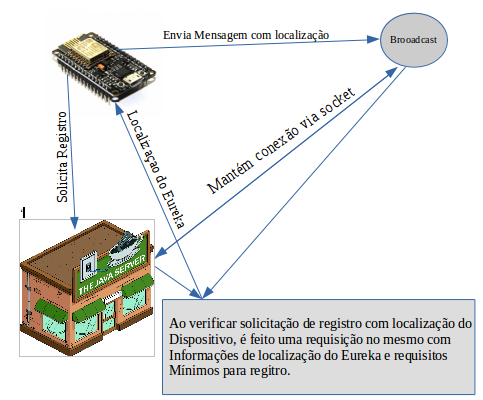
\includegraphics[height=6.2cm]{comunicacao}
\caption{Comunicação entre o dispositivo e o EurekaServer \cite{imagemjavaserver}.}
\label{fig:hystrix-container}
\end{figure}

A figura \ref{functtentregistroeureka} demonstra a primeira função. Este função foi dividida em três funções menores. Uma que registrará o servidor da aplicação, outra que aguardará uma requisição do Eureka Server, e  outra que fará a tentativa de registro.

\begin{figure}[H]
\centering

\begin{lstlisting}
  function startEureka()
    registerServer()
    waitRegister()
    tryingToRegister()
  end
\end{lstlisting}
\caption{Função de tentativa de registro.}
\label{functtentregistroeureka}
\end{figure}
  
Assim que o dispositivo receber a requisição do Eureka Server, será feito uma verificação dos parâmetros, em busca do parâmetro ip, onde conterá o endereço do servidor. Isto pode ser visualizado na figura \ref{waitRegisterFN}. Após o NodeMCU ESP82666 saber onde se encontra o gateway de serviços, será feito o registro no mesmo, e finalizado a conexão do dispositivo no endereço broadcast, conforme a figura \ref{tryingToRegisterFN}. A função que contém o protocolo para registra no Eureka Server pode ser visualizada na figura \ref{protocolojsoneureka}, e a função que criará um pequeno servidor para controle dos pinos digitais pode ser visto na figura \ref{servergpio}.

\section{Resultados}
Neste trabalho foi feito a integração entre um dispositivo IoT com módulo WiFi e um micro-serviço. Foi utilizado  \emph{Broadcast} e \emph{Socket}, para que o EurekaServer observasse a rede, para que quando recebesse uma mensagem de algum dispositivo, fosse feito a requisição para o mesmo, para que o dispositivo tivesse as informações necessárias para registro da aplicação.   

\section{Conclusões e trabalhos futuros}
Considerando a arquitetura que foi desenvolvida, foi possível ser feita esta integração, e o dispositivo conseguiu se registrar no EurekaServer. Fácil configuração dos dispositivos e dos micro-serviços é algo plausível para preenchimento da lacuna deste trabalho. Sendo assim, foram abertas possibidades para desenvolvimento de outros serviços que se integrem com os dispositivos de forma recíproca. Para trabalhos futuros, é viável o desenvolvimento de dispositivos que tenham funções coesas, seguindo o padrão de arquitetura dos micro-serviços. De tal forma, se os micro-serviços e os dispositivos trabalhem de forma independente, torna-se fácil a manutenção de cada serviço ou dispositivo sem afetar os demais.

\newpage
\appendices

\section{Início da thread}

\begin{figure}[H]
\centering

\begin{lstlisting}[language=Java]
  @SpringBootApplication
  @EnableEurekaServer
  @RestController
  @RequestMapping("/")
  public class Application {
      public static void main(String[] args) 
        throws InterruptedException {

          Thread thread = new Thread(() -> {
              System.out.println("----->  thread");
              Server server = new Server();
              server.run();
          });

          thread.start();

          SpringApplication.run(Application.class, args);
      }

      @RequestMapping(value = "send-server", 
        method = RequestMethod.GET)
      public String sendServer() {
          return "Server send!";
      }
  }
\end{lstlisting}
\caption{Início da thread no Eureka Server}
\label{broadcasteureka}
\end{figure}

\section{Espera por registro}

\begin{figure}[H]
\centering

\begin{lstlisting}
  function waitRegister()
  local srvConfigure = net.createServer(net.TCP, 0)
    srvConfigure:listen(
    8000,
    function(conn)
      conn:on(
      "receive",
      function(conn, request)
        print(request)
        local buf = "ok";
        local index = 
            string.find(request, "?ip=")
        local novo = string
            .sub(request, index)
        local ip = string
            .match(novo, "%d+%.%d+%.%d+%.%d+%:*%d*")

        if (ip ~= nil) then
          registered = true
          registerEureka(wifi.sta.getip(), "http://"..ip)
        end

        conn:send(buf);
        conn:close();
        collectgarbage();
      end)
      end)
  end
\end{lstlisting}
\caption{Espera do Eureka Server.}
\label{waitRegisterFN}
\end{figure}


\section{Registro no Eureka}
\begin{figure}[H]
\centering

\begin{lstlisting}
  function tryingToRegister()
    local registered = false
    timeout = 0
    tmr.alarm(2, 1000, 1,
      function()
          if wifi.sta.getip() == nil 
            and wifi.sta.getbroadcast() == nil then
            print("IP unavaiable, waiting... " .. timeout)
            timeout = timeout + 1
            if timeout >= 20 then
              print("Deleting configuration...")
              file.remove("config.lc")
              node.restart()
            end
          else
          if (pcall(function()
            ulala = net.createConnection(net.UDP, 0)
            ulala:send(1234, wifi.sta
              .getbroadcast(), "Request Address Eureka")
            tmr.alarm(3, 1000, 1, function()
              if registered == false then
                print("Trying to register...")
                local ulala = net.createConnection(net.UDP)
                ulala:send(1234, wifi.sta.getbroadcast(), 
                  "Request Address Eureka"..tostring(math.random(1,1000)))
                ulala:close()
                ulala = nil
              else
                tmr.stop(3)
              end
            end)
          end)) then
            print("Send register to Broadcast...")
          else
            print("Error to send register in Broadcast...")
          end
          
          print("Connected, IP is " .. wifi.sta.getip())
          tmr.stop(2)
          end
        end
    )
  end
\end{lstlisting}
\caption{Registro no Eureka.}
\label{tryingToRegisterFN}
\end{figure}

\clearpage

\section{Socket com Broadcast}

\begin{figure}[H]
\centering

\begin{lstlisting}[language=Java]
  public class Server {

    public static final int DEFAULT_PORT = 1234;
    private DatagramSocket socket;
    private DatagramPacket packet;

    public void run() {
        try {
            socket = new DatagramSocket(DEFAULT_PORT);
        } catch (Exception ex) {
            System.out.println("Problem creating socket on port: " 
              + DEFAULT_PORT);
        }

        packet = new DatagramPacket(new byte[1], 1);

        while (true) {
          try {
            socket.receive(packet);
            System.out.println("Received from: " 
              + packet.getAddress() + ":" + packet.getPort());
            byte[] outBuffer = new java
              .util.Date().toString().getBytes();
            packet.setData(outBuffer);
            packet.setLength(outBuffer.length);
            socket.setBroadcast(true);
            socket.send(packet);

            Set<InetAddress> localAddress = getLocalAddress();

            Set<String> ips = localAddress.stream()
                    .map(ad -> ad.getHostAddress())
                    .collect(Collectors.toSet())
                    .stream().sorted()
                    .collect(Collectors.toSet());

            RestTemplate template = new RestTemplate();

            ips.forEach(ip -> {
                try {
                    template.exchange("http://" 
                    + packet.getAddress().getHostAddress()
                    .concat(":8000?ip={ip}"),
                            HttpMethod.GET,
                            HttpEntity.EMPTY,
                            Void.class,
                            ip.concat(":8000"));
                } catch (Exception e) {
                    e.printStackTrace();
                }
            });

            System.out.println("Message ----> " + packet
              .getAddress().getHostAddress());
          } catch (IOException ie) {
            ie.printStackTrace();
          }
        }
    }
  }
\end{lstlisting}
\caption{Socket com Broadcast}
\label{broadcastcodejava}
\end{figure}

\section{Protocolo para registro no Eureka Server}
\begin{figure}[H]
\centering

\begin{lstlisting}
  function registerEureka(ip, addressEureka)
    print("Registering on Address Eureka "..addressEureka.." the ip "..ip)
    http.post(
    addressEureka.."/eureka/apps/appID",
    "Content-Type: application/json\r\n",
    [[{
    "instance": {
      "hostName": "]]..ip..[[",
      "app": "]].."NodeMcuEsp8266"
        ..node.chipid()..[[",
      "ipAddr": "http://]]..ip..[[",
      "status": "UP",
      "port": {
        "@enabled": "true",
        "$": "8080"
      },
      "securePort": {
        "@enabled": "false",
        "$": "443"
      },
      "dataCenterInfo": {
        "@class": "com.netflix.appinfo
          .InstanceInfo$DefaultDataCenterInfo",
        "name": "MyOwn"
      },
      "leaseInfo": {
        "renewalIntervalInSecs": 30,
        "durationInSecs": 90,
        "registrationTimestamp": 1492644843509,
        "lastRenewalTimestamp": 1492649644434,
        "evictionTimestamp": 0,
        "serviceUpTimestamp": 1492644813469
      },
      "homePageUrl": "http://]]..ip..[[:8080/",
      "statusPageUrl": "http://]]..ip..[[:8080/info",
      "healthCheckUrl": "http://]]..ip..[[:8080/health",
      "vipAddress": "]].."NodeMcuEsp8266"..node.chipid()
      ..[["}}]],
    function(code, data)
        if (code < 0) then
            print("HTTP request failed")
        else
            gpio.mode(4, gpio.OUTPUT)
            gpio.write(4, gpio.LOW)
            print(code, data)
        end
    end)
  end

\end{lstlisting}
\caption{JSON Eureka}
\label{protocolojsoneureka}
\end{figure}

\clearpage

\section{Servidor para controle GPIO}
\begin{figure}[H]
\centering
\begin{lstlisting}
  function registerServer()
    srv:listen(
      8080,
      function(conn)
        conn:on("receive", function(client,request)
          local buf = [[
          <!DOCTYPE html>
          <html lang="pt-br">
          <head>
          <meta charset="UTF-8">
          <title>NodeMcu ESP8266</title>
          </head>
          <body>
          ]];
          local _, _, method, 
          path, vars = string
          .find(request, "([A-Z]+) (.+)?(.+) HTTP");
          if(method == nil)then
            _, _, method, path = 
            string.find(request, "([A-Z]+) (.+) HTTP");
          end
          local _GET = {}
          if (vars ~= nil)then
            for k, v in string
              .gmatch(vars, "(%w+)=(%w+)&*") do
                _GET[k] = v
            end
          end
          buf = buf.."<h1> ESP8266 Web Server</h1>";
          for i=1,8,1
          do
              gpio.mode(i, gpio.OUTPUT)
              buf = buf.."<p>DIGITAL "..i
              .." <a href=\"?pin="..i.."&stat=on\">
                    <button>ON</button>
                  </a>&nbsp;
                  <a href=\"?pin="..i.."&stat=off\">
                  <button>OFF</button></a></p>"
          end

          if (_GET.stat ~= nil and _GET.stat ~= nil) then
              if (_GET.stat == "on") then
                  gpio.write(_GET.pin, gpio.HIGH);
              else
                  gpio.write(_GET.pin, gpio.LOW);
              end
          end

          buf = buf..[[
              </body>
              </html>
          ]]

          print(buf)
          
          client:send(buf);
        end)
          
        conn:on(
            "sent",
            function(conn)
                conn:close();
                collectgarbage();
            end)
      end)
  end  
\end{lstlisting}
\caption{Servidor GPIO}
\label{servergpio}
\end{figure}


% Can use something like this to put references on a page
% by themselves when using endfloat and the captionsoff option.
\ifCLASSOPTIONcaptionsoff
  \newpage
\fi



% trigger a \newpage just before the given reference
% number - used to balance the columns on the last page
% adjust value as needed - may need to be readjusted if
% the document is modified later
%\IEEEtriggeratref{8}
% The "triggered" command can be changed if desired:
%\IEEEtriggercmd{\enlargethispage{-5in}}

% references section

% can use a bibliography generated by BibTeX as a .bbl file
% BibTeX documentation can be easily obtained at:
% http://mirror.ctan.org/biblio/bibtex/contrib/doc/
% The IEEEtran BibTeX style support page is at:
% http://www.michaelshell.org/tex/ieeetran/bibtex/
%\bibliographystyle{IEEEtran}
% argument is your BibTeX string definitions and bibliography database(s)
%\bibliography{IEEEabrv,../bib/paper}
%
% <OR> manually copy in the resultant .bbl file
% set second argument of \begin to the number of references
% (used to reserve space for the reference number labels box)
\begin{thebibliography}{1}

\bibitem{freiregebaraiot}
Willian Marques Freire. Munif Gebara Júnior. \emph IoT - A Internet das coisas, vol. 1, 2017

\bibitem{freiregebaramicroservico}
Willian Marques Freire. Munif Gebara Júnior. \emph IoT - Micro-serviços, vol. 1, 2017

\bibitem{PedroZambarda}
Pedro Zambarda. \emph 'Internet das Coisas': entenda o conceito e o que muda com a tecnologia. 2014 [Online] Disponível: http://www.techtudo.com.br/noticias/noticia/2014/08/internet-das-coisas-entenda-o-conceito-e-o-que-muda-com-tecnologia.html [Acesso: 11-Mai-2017]

\bibitem{eurekanetflix}
Netflix. \emph Eureka at a glance. 2014 [Online] Disponível: 
https://github.com/Netflix/eureka/wiki/Eureka-at-a-glance
[Acesso: 26-Jun-2017]

\bibitem{Finep}
Finep. \emph Kevin Ashton – entrevista exclusiva com o criador do termo “Internet das Coisas”, 2015 [Online] Disponível: http://finep.gov.br/noticias/todas-noticias/4446-kevin-ashton-entrevista-exclusiva-com-o-criador-do-termo-internet-das-coisas. [Acesso: 13-Jan-2017]

\bibitem{RicardoFeltrin}
Ricardo Feltrin. \emph Netflix fatura R\$ 1,1 bi no Brasil e ultrapassa o SBT, 2016 [Online] Disponível: https://tvefamosos.uol.com.br/noticias/ooops/2016/01/11/netflix-fatura-r-11-bi-no-brasil-e-ultrapassa-o-sbt.htm. [Acesso: 01-Mai-2017]

\bibitem{SmartBear}
SmartBear. \emph NETFLIX E O SEU SUCESSO COM APIS, 2016 [Online] Disponível: http://mundoapi.com.br/materias/netflix-e-o-seu-sucesso-com-apis. [Acesso: 20-Fev-2017] 

\bibitem{manutayal2016}
Manu Tayal. \emph IoT and Microservices Architecture. [Online] Disponível: http://www.happiestminds.com/blogs/iot-and-microservices-architecture. 2016 [Acesso: 25-Abr-2017]

\bibitem{idc2017}
IDC. \emph Connecting the IotT: The road to success. 2016 [Online] Disponível: http://www.idc.com/infographics/IoT. [Acesso: 15-Fev-2017]

\bibitem{martinfowleretal}
Martin Fowler et al. \emph Microservices. 2014 [Online] Disponível: https://www.martinfowler.com/articles/microservices.html. [Acesso: 20-Mai-2017]

\bibitem{lillianhiper}
Lúcia Leão. \emph O labirinto da hipermídia: arquitetura e navegação no ciberespaço. 1997 [Online]
Disponível:
http://www.alvarestech.com/lillian/Pos-graduacao/Hipermidia.pdf. [Acesso: 01-Jul-2017]


\bibitem{oficinahttp}
Marcos Elias. \emph O que é FTP? E HTTP? 2010 [Online]
Disponível: http://www.explorando.com.br/ftp-http. [Acesso: 01-Jul-2017]

\bibitem{fieldingrest}
Roy Thomas Fielding. \emph Representational State Transfer (REST) 2000 [Online] Disponível: http://www.ics.uci.edu/\~fielding/pubs/dissertation/rest\_arch\_style.htm.
[Acesso: 01-Jul-2017]

\bibitem{pedropintosocket}
Pedro Pinto. \emph Redes – Sabe o que são sockets de comunicação? (Parte I) 2012 [Online] Disponível: https://pplware.sapo.pt/tutoriais/networking/redes-sabe-o-que-sao-sockets-de-comunicacao-parte-i.

\bibitem{tecmundothread}
Fábio Jordao. \emph O que são threads em um processador? 2011 [Online] Disponível: https://www.tecmundo.com.br/9669-o-que-sao-threads-em-um-processador-.htm

\bibitem{jsonpt}
Ecma international. \emph The JSON Data. 2013 [Online] 
Disponível: http://www.ecma-international.org/publications/files/ECMA-ST/ECMA-404.pdf

\bibitem{Sasang}
Sasang Balachandran. \emph General Purpose
Input/Output (GPIO), vol. 1, 2009

\bibitem{imagemjavaserver}
Simpsons Wikia. \emph The Java Server 2017. [Online]
Disponível: http://simpsons.wikia.com/wiki/The\_Java\_Server

\end{thebibliography}

\clearpage

% biography section
% 
% If you have an EPS/PDF photo (graphicx package needed) extra braces are
% needed around the contents of the optional argument to biography to prevent
% the LaTeX parser from getting confused when it sees the complicated
% \includegraphics command within an optional argument. (You could create
% your own custom macro containing the \includegraphics command to make things
% simpler here.)
%\begin{IEEEbiography}[{\includegraphics[width=1in,height=1.25in,clip,keepaspectratio]{mshell}}]{Michael Shell}
% or if you just want to reserve a space for a photo:

\begin{IEEEbiography}[{
\includegraphics[width=1in,height=1.25in,clip,keepaspectratio]{willian}}]{Willian Marques Freire}
Possui Ensino Médio completo pelo Colégio Estadual Rosa Delúcia Calsavara (2013). Atualmente é Desenvolvedor de Software da Gumga Tecnologia da Informação S/A. Tem experiência na área de Ciência da Computação.
\end{IEEEbiography}

\begin{IEEEbiography}[{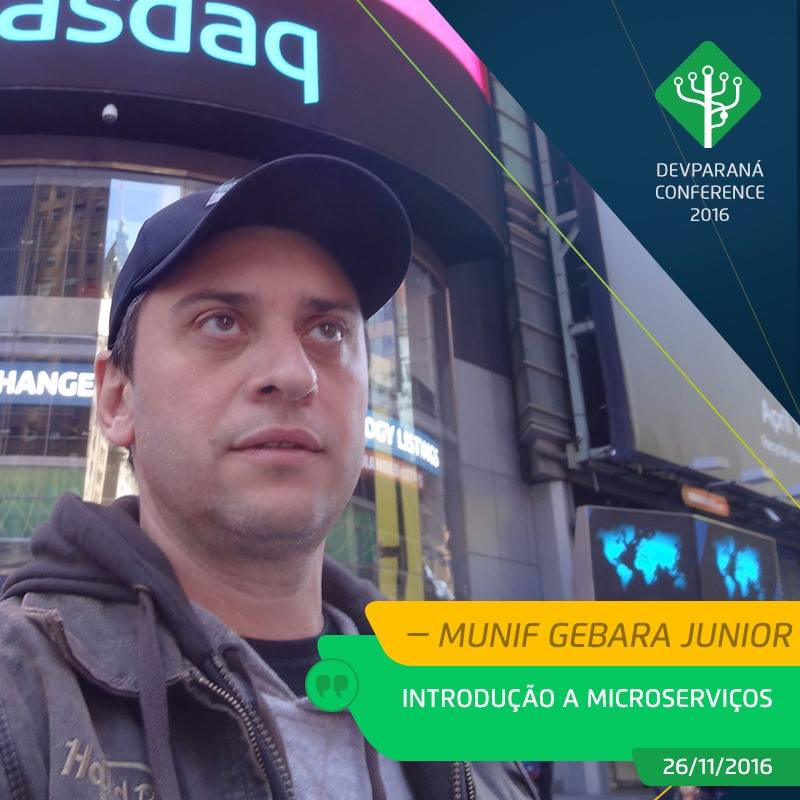
\includegraphics[width=1in,height=1.25in,clip,keepaspectratio]{munif}}]{Munif Gebara Júnior}
Possui graduação em Ciência da Computação pela Universidade Estadual de Maringá (1997) e mestrado em Engenharia Elétrica e Informática Industrial pela Universidade Tecnológica Federal do Paraná (2001). Atualmente é professor da Fundação Faculdade de Filosofia Ciências e Letras de Mandaguari e professor de ensino superior da Faculdade de Tecnologia e Ciências do Norte do Paraná Ltda e desenvolvedor.
\end{IEEEbiography}

\end{document}


